\documentclass[a0h]{btrpstr}

% Please read the vertical demo for more useful comments,
% this is given just as it is.

\usepackage{fontspec}
\setmainfont{FiraSansLight}[
  ItalicFont=FiraSansLightItalic,
  BoldFont=FiraSansBold,
  BoldItalicFont=FiraSansBoldItalic]
\setmonofont{FiraMono}

\usetikzlibrary{positioning}

\usepackage{pgfplots}
\usepackage{qrcode}
\usepackage{lipsum}

\begin{document}
\begin{poster}[fontsizes=32pt]
\posterbackground{fill=white}

\node[text width=.4\paperwidth,text=white,font=\fontsize{2.5in}{2.5in}\selectfont]
  (leader) at (poster.center)
  {This really helps a lot with the design of the \textbf{\#betterposter}s.};
\node[below=of leader.south east,anchor=north east,color=white]
  (note) {\textit{--- a compendium of \TeX{}nicians, 2020}};
\posterboxbackground{leaderbg}
  {(leader)(note)(leader|-poster.north)(leader|-poster.south)}
  {inner sep=3in,shade,top color=cyan!40!black,bottom color=black}
\node[anchor=south west,fill=white]
  (qrcode) at ([yshift=2in] poster.south-|leader.west)
  {\qrcode[height=4in]{https://github.com/exaexa/btrpstr}};
\node[anchor=base west, font=\tt\footnotesize, text=white] at([xshift=1em] qrcode.south east)
  {https://github.com/exaexa/btrpstr};

\newpostercol{left}{
  start={([xshift=2em] poster.north west)},
  span={([xshift=-2em] leaderbg.west)}}
\newpostercol{right}{
  start={([xshift=2em] leaderbg.east|- poster.north)},
  span={([xshift=-2em] poster.east)}}

\begin{posterbox}{titlebox}{col=left,offset=2em,sep=0pt}
  {\hyphenpenalty=10000\Large\bfseries A better \LaTeX{} poster template, now with Ti{\it k}Z
  features and a~bit of support for really long headings\par}

  Author First, Second Author

  \texttt{\{author,second\}@insti.tute.tld}

  \scriptsize Department of Poster Engineering, Great University, City
\end{posterbox}

\begin{posterbox}{stickynote}{col=left, below=titlebox, offset=3ex, style={color=yellow!50!orange!80!black, fill=yellow!25},sep=1em}
  \Large This is the main message of the whole poster!
  \bfseries Looks like a sticky note!
\end{posterbox}

\begin{posterbox}{whitebox}{col=left, below=stickynote, offset=1ex}
  \lipsum[1][1-4]
\end{posterbox}

\begin{headerbox}{hbox}{col=left, below=whitebox, offset=1ex, header style={fill=cyan!20!black, text=white}, body style={fill=cyan!20}, header={A box, now with a header}}
  \lipsum[2]
\end{headerbox}

\begin{posterbox}{logo}{col=left, below=hbox, offset=3ex}
  \resizebox{\linewidth}{!}{$\alpha\choose\omega$}
\end{posterbox}

\begin{posterbox}{plot}{col=right, offset=2em}
  \lipsum[1][4-6]

  \vspace{2ex}
  \centering
  \pgfplotsset{width=0.5\linewidth}
  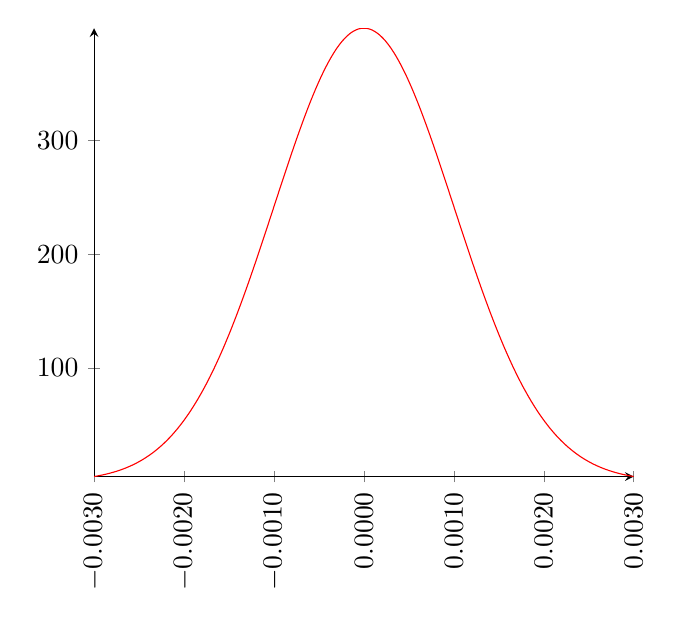
\begin{tikzpicture}
  \begin{axis}[axis lines=left, scaled ticks=false, xticklabel style={ rotate=90, anchor=east, /pgf/number format/precision=4, /pgf/number format/fixed, /pgf/number format/fixed zerofill, }, ]
  \newcommand\MU{0}
  \newcommand\SIGMA{1e-3}
  \addplot [red,domain=-3*\SIGMA:3*\SIGMA,samples=201]
    {exp(-(x-\MU)^2 / 2 / \SIGMA^2) / (\SIGMA * sqrt(2*pi))};
  \end{axis}
  \end{tikzpicture}
\end{posterbox}

\begin{posterbox}{bgtest}{col=right,below=plot,offset=3cm}
  \lipsum[2]
\end{posterbox}

\posterboxbackground{testbg}
  {(bgtest)(bgtest-|poster.east)}
  {inner sep=1cm, fill=green!66!yellow!10}

\end{poster}
\end{document}
